\chapter{Rotor FE}
\section{Beam Element FE Equation}
\subsection{Bernoulli-Euler Beam equation}
Assumptions used to derive the bernoulli-Euler beam equation are (Complete derivation in \cite{craig2006fundamentals}):
\begin{enumerate}
	\item Beam is bending in a plane, in this case in the z-direction, where the x-direction is along the length of the beam.
	\item The  neutral axis undergoes no deformation in the longitudinal direction.
	\item Cross sections remain plane and perpendicular to the nuetral axis.
	\item The material is linear-elastic.
	\item Stresses in the z and y direction are negligible compared to those in the x direction.
	\item Rotatory inertia may be neglected in moment equation.
	\item Mass density is constant at each cross section, so that each mass center is coicident with the centroid of that section.
\end{enumerate}
Using kinematics and assumptions 2 \& 3, the strain in the x direction may be related to the curvature of the beam, $\mu(x,t)$, and the distance from the neutral axis by
\begin{equation} \label{eq:curvature}
\epsilon=-\dfrac{y}{\mu}
\end{equation}
Then, with assumption 4 \& 7 the relation from curvature to moment is
\begin{equation}
M(x,t)=\dfrac{EI}{\mu}
\end{equation}
\begin{figure}
	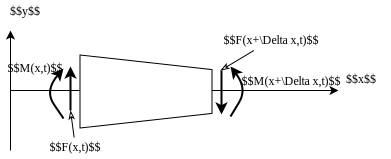
\includegraphics[]{figures/BeamFBD.pdf}
	\caption{electrical Diagram}
	\label{fig:diagram}
\end{figure}
\begin{equation} \label{eq:FEGoverning}
u(x,y,z,t)=N(x,y,z)q(t)
\end{equation}